Multiple choice section. All points are for choosing the correct answer. No justification is needed.
\begin{questions} 

\question[3] A parabola has a vertex of $(-3,2)$, and the vertex is a maximum. What is a possible equation for the parabola?
\begin{checkboxes}

    \choice $y=(x+3)^2+2$
    \choice $y=-(x-3)^2-2$
        \choice $y=-(x+3)^2+2$
    \choice $y=-(x-2)^2-3$
    \choice None of the above.
\end{checkboxes}

\question[3] The graph below has which properties?

    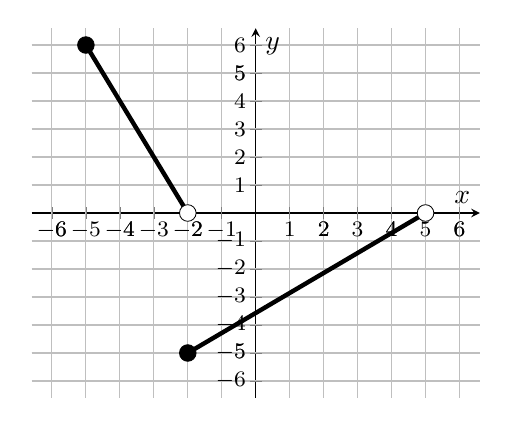
\begin{tikzpicture}
\begin{axis}[
   grid = major,
   extra x ticks={-6,-5,-4,-3,-2,-1,1,2,3,4,5,6},
   extra y ticks={-6,-5,-4,-3,-2,-1,1,2,3,4,5,6},
   %xminorgrids=true,
   width=.6\textwidth,
   %clip = true,
   %clip mode=individual,
   %restrict y to domain=-12:12,
   axis x line = middle,
   axis y line = middle,
        yticklabel style = {font=\footnotesize,xshift=0.5ex},
        xticklabel style = {font=\footnotesize,yshift=0.5ex},
   xlabel={$x$},
   %xlabel style={at=(current axis.right of origin)},
   ylabel={$y$},
   %ylabel style={at=(current axis.above origin)},
   %domain = -5:5,
   xmin = -6,
   xmax = 6,
   enlarge y limits={rel=0.05},
   enlarge x limits={rel=0.05},
   ymin = -6,
   ymax = 6,
 ]
\addplot[smooth, ultra thick, domain = -5:-2,samples=2
	] { (-2*x)-4}
 node[pos=.95](endofplotsquare){} ;
 \addplot[smooth, ultra thick, domain = -2:5,samples=2
	] { (5/7)*(x+2)-5}
 node[pos=.95](endofplotsquare){} ;
%\node [right] at (endofplotsquare) {$f(x)$};%
        \addplot[only marks,mark=*, mark options={scale=2, fill=white}, line width=0.3pt, mark size=1.5pt] coordinates{(-2,0) (5,0)};
        \addplot[only marks,mark=*, mark options={scale=2, fill=none}, line width=0.3pt, mark size=1.5pt] coordinates{(-5,6) (-2,-5)};
\end{axis}
\end{tikzpicture}
\begin{checkboxes}
    \choice The graph is a function and does have an inverse.
    \choice The graph is neither a function nor has an inverse.
    \choice The graph is not a function, but does have an inverse.
    \choice The graph is a function, but does not have an inverse.

    \choice None of the above.
\end{checkboxes}

\question[3] Consider a polynomial
\[P(x) = ax^n\]
You know $n$ is a positive integer, but do not know $a$. If as $x\to-\infty$ $P(x)\to-\infty$ and as $x\to+\infty$ $P(x)\to-\infty$. What do you know about $a$ and $n$?
\begin{checkboxes}
    \choice $a$ is positive and $n$ is odd.
    \choice $a$ is negative and $n$ is odd.
        \choice $a$ is negative and $n$ is even.
    \choice $a$ is positive and $n$ is even.

    \choice None of the above.
\end{checkboxes}

\newpage
\question[3] A graph of a generic quadratic $y=ax^2+bx+c$, with $a\neq0$
\begin{checkboxes}
    \choice will always touch (intersect) the $x$-axis in 2 different places.
    \choice will always touch (intersect) the $x$-axis at least once.
    \choice will always touch (intersect) the $x$-axis exactly once.
    \choice may not touch (intersect) the $x$-axis at all.
    \choice None of the above.
\end{checkboxes}

\question[3] A graph of a generic quadratic $y=ax^2+bx+c$, with $a\neq0$
\begin{checkboxes}
    \choice will always touch (intersect) the $y$-axis in 2 different places.
    \choice will always touch (intersect) the $y$-axis at least once.
    \choice will always touch (intersect) the $y$-axis exactly once.
    \choice may not touch (intersect) the $y$-axis at all.
    \choice None of the above.
\end{checkboxes}



\newpage
\question %
Ed wants to build a rectangular pen for his sheep, and he wants to make the pen have the largest possible area. Ed has 40 feet worth of fencing available. 

\begin{parts}%[label=(\alph*)]
    \part[4] Let $x$ denote the length of the horizontal side. Express the area $A$ in terms of $x$.
    \vspace{8cm}
    \part[6] Using the expression obtained in (a), find the value of $x$ that maximizes $A$, the area of the pen, and find this maximal area.
\end{parts}

\newpage


% \hspace{-.5in}Free answer section. Work must be shown to get credit for any answer. Partial credit may be given even for incorrect final answers, so show your work.

%\newpage

\question[10] %\textbf{[Section 3.3]} 
Find the quotient and remainder of the following:
$$(8x^4+2x^3-10x^2+4)\div (2x^2-1)$$

\newpage

\question[10] %\textbf{[Section 2.6]} 
The graph of a function $y = f(x)$ is displayed below:

\begin{center}
    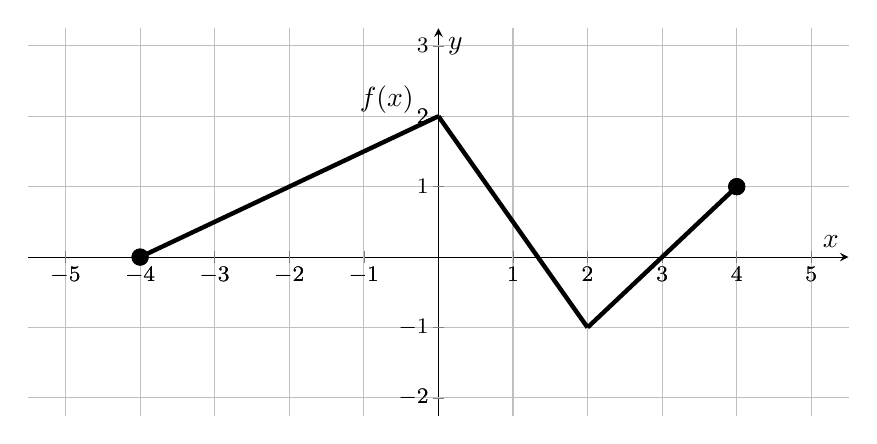
\begin{tikzpicture}
\begin{axis}[
   grid = major,
   extra x ticks={-6,-5,-4,-3,-2,-1,1,2,3,4,5,6},
   extra y ticks={-6,-5,-4,-3,-2,-1,1,2,3,4,5,6},
   %xminorgrids=true,
   width=12cm,
   height=6.5cm,
   %clip = true,
   %clip mode=individual,
   %restrict y to domain=-12:12,
   axis x line = middle,
   axis y line = middle,
        yticklabel style = {font=\footnotesize,xshift=0.5ex},
        xticklabel style = {font=\footnotesize,yshift=0.5ex},
   xlabel={$x$},
   %xlabel style={at=(current axis.right of origin)},
   ylabel={$y$},
   %ylabel style={at=(current axis.above origin)},
   %domain = -5:5,
   xmin = -5,
   xmax = 5,
   enlarge y limits={rel=0.05},
   enlarge x limits={rel=0.05},
   ymin = -2,
   ymax = 3,
 ]
 \addplot[smooth, ultra thick, domain = -4:0,samples=2
	] { .5*x+2}
 node[pos=.95](endofplotsquare){} ;
\node [above left] at (endofplotsquare) {$f(x)$};%
 \addplot[smooth, ultra thick, domain = 0:2,samples=2
	] { -(3/2)*x+2};
  \addplot[smooth, ultra thick, domain = 2:4,samples=2
	] { x-3};
        \addplot[only marks,mark=*, mark options={scale=2, fill=none}, line width=0.3pt, mark size=1.5pt] coordinates{(-4,0) (4,1)};
\end{axis}
\end{tikzpicture}
    
    % \includegraphics[scale=1.5]{Midterm2/figures/transform.jpg}
\end{center}

Draw the graph of $y = -f(2x) - 1$ below.

    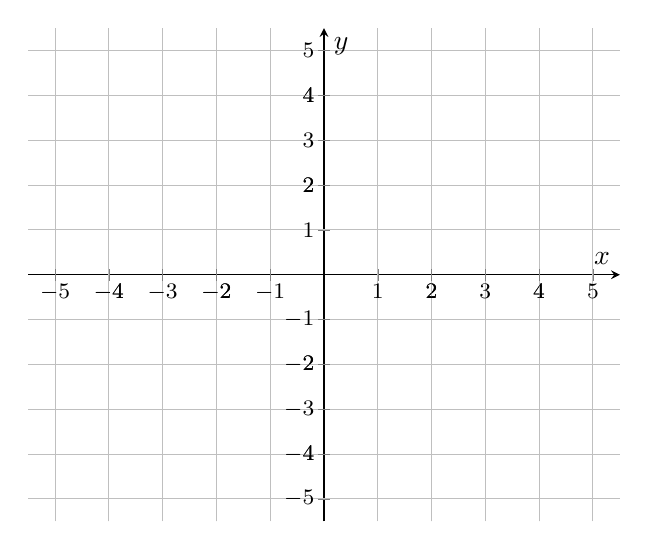
\begin{tikzpicture}
\begin{axis}[
   grid = major,
   extra x ticks={-6,-5,-4,-3,-2,-1,1,2,3,4,5,6},
   extra y ticks={-6,-5,-4,-3,-2,-1,1,2,3,4,5,6},
   %xminorgrids=true,
   width=.75\textwidth,
   %clip = true,
   %clip mode=individual,
   %restrict y to domain=-12:12,
   axis x line = middle,
   axis y line = middle,
        yticklabel style = {font=\footnotesize,xshift=0.5ex},
        xticklabel style = {font=\footnotesize,yshift=0.5ex},
   xlabel={$x$},
   %xlabel style={at=(current axis.right of origin)},
   ylabel={$y$},
   %ylabel style={at=(current axis.above origin)},
   %domain = -5:5,
   xmin = -5,
   xmax = 5,
   enlarge y limits={rel=0.05},
   enlarge x limits={rel=0.05},
   ymin = -5,
   ymax = 5,
 ]

\end{axis}
\end{tikzpicture}
% \begin{center}
%     \includegraphics[scale=0.9]{Midterm2/figures/transform_2.png}
% \end{center}



\newpage
%Ang 2.8

\question Let $f(x)=\dfrac{x+5}{2x-3}$.
\begin{parts}
    \part[4] Find the domain of $f$.
    \vspace{8cm}
    \part[6] Find $f^{-1}(x)$.
    \vspace{8cm}
\end{parts}

\newpage

\question A box maker can produce 100 boxes every 4 hours. They start one morning with 75 boxes already made. 

\begin{parts}
    \part[3] What is the hourly rate of production (with correct units)?\vspace{5cm}
    \part[4] Write the equation for the number of boxes  after $x$ hours that day?
    \vspace{6cm}
    \part[3] How many hours have to pass before they have  300 boxes that day?
\end{parts}


\newpage

%Logan 3.2
\question Let $f(x)=2(x+2)(x-2)(x-5)^2$ be a polynomial function.
\begin{parts}
    

    \part[2] Fill in the blanks with the end behavior of $f(x)$ (no justification needed):\vspace{.5cm}
    
    As $x\to -\infty$, $y\to$ \underline{\qquad\qquad}.\vspace{.5cm}
    
    As $x\to +\infty$, $y\to$ \underline{\qquad\qquad}.
    \part[4] Write the $x$-intercepts (zeros) of the function $f(x)$.
    \vspace{0.5in}
    \part[4] Using your answers to parts (a) and (b), sketch the graph of $f(x)$ on the $xy$-plane provided below. Clearly indicate the $x$-intercepts of $f(x)$.
\end{parts}

\begin{center}
    \begin{tikzpicture}[scale=2]
    % Draw x-axis
    \draw[->,thick] (-3,0) -- (3,0) node[right] {$x$};
    % Draw y-axis
    \draw[->,thick] (0,-3) -- (0,3) node[above] {$y$};
\end{tikzpicture}
\end{center}

\newpage
\question %\textbf{[Section 3.4\&3.5]} 
Let $f(x) = 2x^{3}-x^{2}-7x+6$.
\begin{parts}
\part[2] What are all the possible rational roots of $f(x)$ according to the rational root theorem?
\vspace{3cm}

\part[8] If we know that $f(x)$ has a root at $x=1$, find all the roots of $f(x)$
\vspace{12cm}

\part[2] Write $f(x)$ as a product of linear factors.
\end{parts}
\end{questions}